\documentclass{report}
\usepackage[T1]{fontenc}
\usepackage[utf8]{inputenc}
\usepackage[backend=biber, style=ieee]{biblatex}
\usepackage{csquotes}
\usepackage[portuguese]{babel}
\usepackage{blindtext}
\usepackage[printonlyused]{acronym}
\usepackage{hyperref}
\usepackage{graphicx}
\usepackage{indentfirst}
\usepackage{float}
\usepackage{subcaption}

\bibliography{bibliografia}
\setlength{\parskip}{0.35em}

\begin{document}
%%% DEFINIÇÕES GLOBAIS %%%
\def\titulo{Realidade Aumentada}
\def\data{Aveiro, dezembro 2021}
\def\autores{Miguel Vila, Diogo Silva}
\def\autorescontactos{(107276) miguelovila@ua.pt, (108212) dsgps@ua.pt}
\def\versao{BETA SINCE 2013}
\def\departamento{DETI}
\def\empresa{UNIVERSIDADE DE AVEIRO}
\def\logotipo{ua.pdf}

%%% ESTRUTURA CAPA %%%
\begin{titlepage}
\begin{center}
\vspace*{50mm}
{\Huge \titulo}\\ 
\vspace{10mm}
{\Large \empresa}\\
\vspace{10mm}
{\LARGE \autores}\\ 
\vspace{30mm}
\begin{figure}[h]
\center
\includegraphics{\logotipo}
\end{figure}
\vspace{30mm}
\end{center}
\begin{flushright}
\versao
\end{flushright}
\end{titlepage}

%%%  PÁGINA DE TÍTULO %%%
\title{%
{\Huge\textbf{\titulo}}\\
{\Large \departamento\\ \empresa}
}
\author{
    \autores \\
    \autorescontactos
}
\date{\data}
\maketitle
\pagenumbering{roman}

%%% RESUMO %%%
\begin{abstract}
!!!TODO!!! Resumo de 200-300 palavras.
\end{abstract}

%%% AGRADECIMENTOS %%%
\renewcommand{\abstractname}{Agradecimentos}
\begin{abstract}
Para este trabalho ser realizado não pudemos dispensar da ajuda dos professores, os quais estiveram sempre recetivos e disponiveis para nos ajudar com qualquer duvida e esclarecimento. Por isso, deixamos aqui o nosso agradecimento especial aos professores da discilpina de \ac{iei}, o professor António Manuel Adrego da Rocha e o professor Óscar Pereira, sem o conhecimento transimitido por eles não conseguiriamos ter elaborado o trabalho colaborativo de maneira tão correta e com todos os recursos que tivemos disponiveis para a construção deste trabalho.
\end{abstract}

\tableofcontents
\listoffigures

\clearpage
\pagenumbering{arabic}

%%% INTRODUÇÃO %%%%
\chapter{Introdução}
\label{chap.introducao}


\begin{quote}
    ``\emph{A display connected to a digital computer gives us a chance to gain familiarity with concepts not realizable in the physical world. It is a looking glass into a mathematical wonderland.}''\cite{Sutherland65theultimate}
\end{quote}
\begin{flushright}
Ivan E. Sutherland
\end{flushright}

Desde os primórdios que o Homem procura ter controlo da sua realidade moldando-a e modificando-a de modo a que as suas necessidades sejam supridas. Pode-se tomar como exemplo o controlo do fogo: quando o Homem primitivo descobriu como gerar artificialmente e controlar o fogo teve a sua vida facilitada e abriu um leque de novas possibilidades que originaram uma grande revolução a todos os níveis.

Passados alguns milhares de anos, o ser humano continua a tentar ter ainda mais controlo sobre a realidade de modo a que o impossível se torne possível. Como a \ac{ra} estende virtualmente aquilo que existe no mundo real, existe uma forte probabilidade de que, tal como o fogo, a \ac{ra} venha a revolucionar a forma como se vive e dar azo ao surgimento de novas possibilidades.

Apesar de ser uma tecnologia relativamente recente, esta tem tido uma considerável evolução por isso, promete ser o futuro da tecnologia e integrar-se cada vez mais no dia a dia do cidadão comum. Atualmente não está implementada em grande escala, mas já tem vastas aplicações a nível empresarial. Áreas como a medicina, o entretenimento, o \textit{design}, a educação e a arquitetura poderão beneficiar dos novos recursos e funcionalidades criados por esta tecnologia.

Além disso, empresas no mercado tecnológico como a \textit{Google}, a \textit{Microsoft} e a \textit{Samsung} apostam no desenvolvimento desta tecnologia que tem potencial para se tornar o “braço-direito” do utilizador no desenvolver da sua atividade profissional e, futuramente, no desenvolvimento da sua vida pessoal. Porém, atualmente apenas a \textit{Microsoft} foi capaz de, com algum sucesso, viabilizar e introduzir estes dispositivos no ambiente industrial e corporativo.

Será que, com todo este investimento e interesse por parte de grandes empresas tecnológicas, esta tecnologia estará à altura para mudar o mundo num futuro próximo?

\section{Objetivos}
Este relatório, realizado no âmbito da unidade curricular de Introdução à Engenharia Informática, terá como principal objetivo dar a conhecer a nova realidade tecnológica dos dispositivos \textit{mixed reality} e a sua utilidade, focando nos óculos holográficos de realidade aumentada \textit{HoloLens 2} desenvolvidos pela \textit{Microsoft}.

Tentar-se-á ainda responder a algumas perguntas frequentes quando o assunto é \ac{ra} tais como: "Será que a \ac{ra} é uma tecnologia relevante?", "A \ac{ra} surgirá no nosso quotidiano num futuro próximo?" e "Quais são as limitações atuais desta tecnologia?"

\section{Organização e estrutura}
O relatório \textit{Realidade Aumentada} contém informação abrangente relativa a esta área e está organizado de forma a que o leitor não necessite de quaisquer conhecimentos prévios para poder acompanhar a totalidade dos capítulos.

O documento encontra-se dividido em 5 capítulos:
\begin{itemize}
    \item No \autoref{chap.introducao} é feita a contextualização do trabalho, explicando o porquê da \ac{ra} ser um tema importante e de interesse. Também são explicitados os objetivos que se pretendem atingir com a leitura do mesmo.
    \item No \autoref{chap.realidade-aumentada} ir-se-á esclarecer o que é a \ac{ra}, perceber como surgiu, explorar possíveis aplicações e alguns exemplos de como a \ac{ra} já está a ser utilizada no quotidiano e ainda conhecer os desafios e limitações que esta tecnologia tem vindo a enfrentar.
    \item No \autoref{chap.oculos-holograficos} é explicado o conceito por detrás dos óculos holográficos. Também se faz um balanço do panorama atual desses dispositivos.
    \item No \autoref{chap.microsoft-hololens-2} analisa-se em detalhe os óculos de realidade aumentada \textit{HoloLens 2} percebendo qual a sua utilidade, quais as suas principais características e a quem se destina.
    \item Por fim, no \autoref{chap.conclusao} serão apresentadas as principais conclusões do trabalho, prevendo de que forma esta tecnologia irá revolucionar e entrar nas vidas do cidadão comum.
\end{itemize}

\section{Metodologia}
Para o presente trabalho, foi utilizada uma metodologia assente na pesquisa exploratória. Esta pesquisa de índole qualitativa baseou-se na recolha de dados de diferentes fontes, tais como artigos, livros, investigações e estudos de referência na área da tecnologia e ciência.

A informação daí recolhida permitiu compreender, aprofundar e consolidar o tema do trabalho, de maneira a apresentá-lo da forma mais clara mais objetiva possível.

%%% REALIDADE AUMENTADA %%%
\chapter{Realidade Aumentada}
\label{chap.realidade-aumentada}
Neste capítulo irá se explicar em que consiste a \ac{ra}, diferenciando-a de tecnologias semelhantes como a \ac{rv} e apresenta-se as diferentes aplicações que a \ac{ra} já tem no quotidiano e que, por muitas vezes, passam despercebidas.

Mostrar-se-á também a sua origem e as diversas etapas que teve que atravessar ao longo dos anos para se tornar na tecnologia que é hoje e apresenta-se alguns exemplos de aplicações no mundo real e exemplos de dispositivos inteligentes que possuem esta tecnologia.

Por fim, explora-se os principais desafios e limitações que a \ac{ra} tem tido e enfrentado.

\section{Conceito}
A \ac{ra} consiste na integração e interligação de elementos ou informações virtuais na visualização do mundo real. É através de dispositivos de entrada como sensores óticos (câmera) e sensores de movimento (giroscópio e acelerómetro) e dispositivos de saída como um écran (convencional ou holográfico) que é feita essa integração do virtual com mundo palpável.

A \ac{ra} é comummente confundida com a \ac{rv} porque, a princípio, podem parecer tecnologias semelhantes, mas, na verdade, existem diversas diferenças entre elas.

Enquanto que a \ac{rv}, tal como o nome indica, pode ser caracterizada pela criação de um ambiente puramente virtual onde o utilizador tenta ter uma experiência imersiva, a \ac{ra} trata-se de uma tecnologia que, através de dispositivos específicos, permite que elementos virtuais interliguem-se e, até mesmo, interajam com a realidade.

Por outras palavras, a \ac{ra} baseia-se numa experiência interativa entre o mundo real e o virtual, onde objetos que pertencem ao plano real podem ser "aumentados" e manipulados no plano virtual e onde objetos pertencentes ao plano virtual podem interagir e moldar-se ao mundo físico.

A \ac{ra} é uma tecnologia abrangente e cheia de possibilidades, por isso, ainda pode ser subdividida em duas outras: a Realidade Mediada e a \ac{rm}. Estas são semelhantes no que toca àquilo que pretendem alcançar, porém usam diferentes técnicas para o fazer:
\begin{itemize}
    \item Na Realidade Mediada, uma câmera capta o ambiente que envolve o utilizador, as imagens obtidas são processadas inserindo os elementos virtuais e, por fim, a imagem é mostrada num écran.
    \item Na \ac{rm}, uns sensores óticos e posicionais mapeiam o ambiente ao redor do utilizador, as posições em que os objetos virtuais aparecerão são processadas e, por fim, os objetos são projetados numa lente transparente dando a noção de profundidade, culminando, assim, numa experiência ainda mais real e imersiva para o utilizador.
\end{itemize}

\begin{figure}[H]
    \centering
    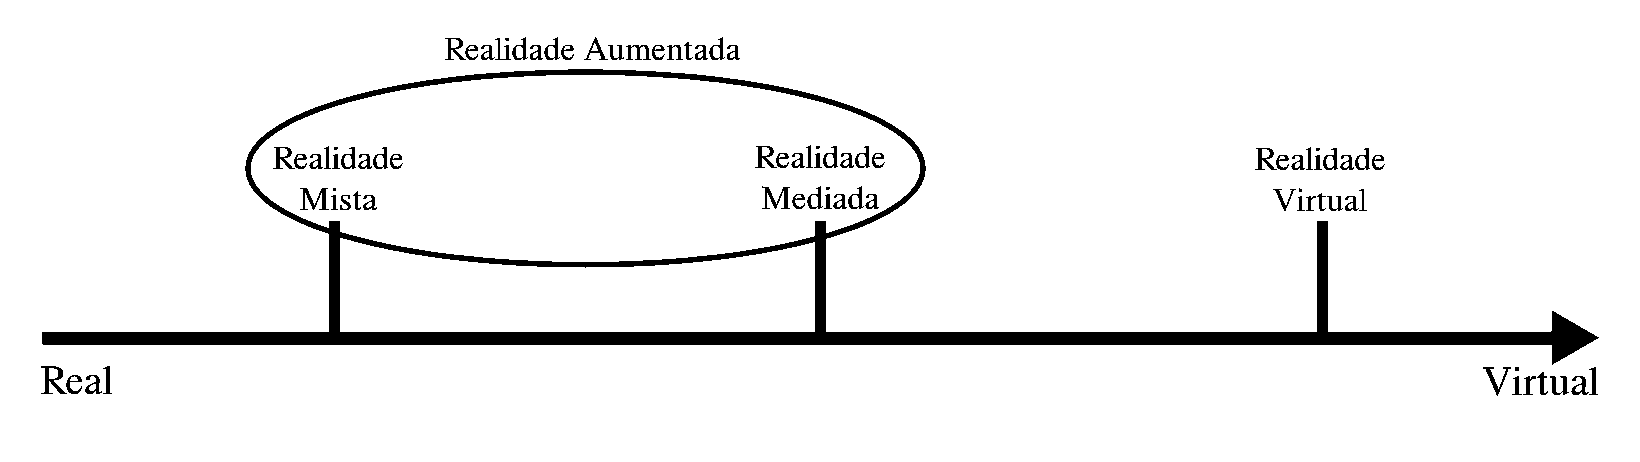
\includegraphics[width=\textwidth]{spectre.png}
    \caption{Espetro de proximidade ao real ou virtual.}
    \label{Fig:spectre}
\end{figure}

Conclui-se então que a \ac{ra} está mais próxima do real do que a \ac{rv} já que esta cria um ambiente totalmente virtual praticamente dissociado do mundo palpável. Conclui-se também que entre a Realidade Mediada e a \ac{rm} esta é aquela que confere um maior grau de imersão ao utilizador.

\section{Origem}
A primeira referência histórica a algo que se assemelha vagamente ao conceito de \ac{ra} data de 1962, quando Morton Heilig inventou uma máquina chamada \textit{Sensorama}. Esta máquina imersiva era capaz de exibir imagens tridimensionais, reproduzir som estéreo, transmitir sensações táteis como vibrações e, ainda, transmitir sensações olfativas.\cite{sousa_ccg_2018}

\begin{figure}
    \centering
    \begin{subfigure}{.5\textwidth}
      \centering
      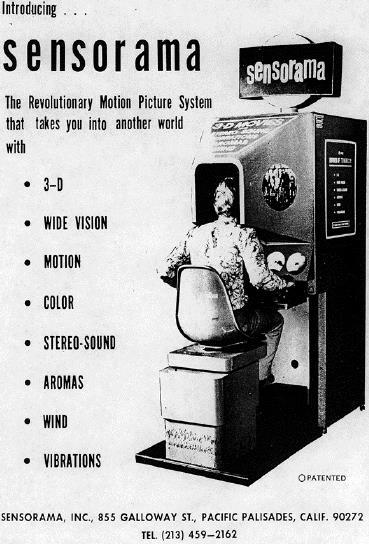
\includegraphics[height=17em]{sensorama.png}
      \label{Fig:sensorama0}
    \end{subfigure}%
    \begin{subfigure}{.5\textwidth}
      \centering
      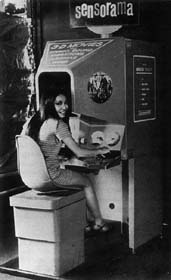
\includegraphics[height=17em]{sensorama1.jpg}
      \label{Fig:sensorama1}
    \end{subfigure}
    \caption{Simulador \textit{Sensorama}}
    \label{Fig:sensorama}
\end{figure}

Este foi o primeiro dispositivo de \ac{rv} que, mesmo não tendo tido financiamento nem apoio na sua época, foi revolucionário e certamente teve impacto no surgimento da \ac{ra} e desenvolvimento da \ac{rv} anos mais tarde.

Já em 1968, Ivan Sutherland, um cientista da computação e também professor universitário, criou com os seus alunos o primeiro \ac{hmd} conectado a um computador que gerava gráficos rudimentares de salas e objetos.\cite{virtualrealitysociety_2020}

Como qualquer outra nova tecnologia, a realidade aumentada surgiu para suprir uma necessidade e foi Thomas Caudell, um cientista e pesquisador da \textit{Boeing}, que em 1992 utilizou pela primeira vez o termo "Realidade Aumentada".

Numa altura em que a \textit{Boeing} estava a produzir em massa um dos maiores e icónicos aviões de todos os tempos, o "\textit{Boeing 747}", Thomas Caudell procurou aumentar a produtividade dos operários da empresa que, de cada vez que necessitavam de fazer uma operação técnica neste avião tinham consultar manuais extensos e de difícil compreensão.

Assim, Thomas teve a ideia de criar um dispositivo, uma espécie de óculos, que auxiliasse os operários que, desta forma, teriam acesso fácil ao manuais e poderiam consultá-los de forma interativa enquanto faziam os procedimentos de manutenção no avião.

\section{Aplicações - Atualidade}
O telemóvel, com a grande qualidade das câmaras que o integram, a precisão dos sensores (giroscópio e magnetómetro) e, também, com o crescente poder de processamento, tornou-se no equipamento ideal e mais conveniente para fazer uso da realidade aumentada.

A \ac{ra} já faz parte do dia a dia de grande parte da população, porém passa despercebida pois está presente em situações que já se consideram algo banais.

Os filtros e efeitos em fotografias e vídeos são o melhor exemplo para demonstrar que a \ac{ra} já chegou a grande parte da população e está presente no dia a dia de qualquer um. A probabilidade de alguém ter experimentado os filtros do \textit{Instagram} ou \textit{Snapchat} pelo menos uma vez é muito alta. Nestes, elementos digitais moldam-se a caras e objetos e interagem dinamicamente com o que é real, sendo um exemplo da implementação da \ac{ra}.

Jogos simples como o famoso \textit{Pokémon GO} ou até mesmo aplicações de grandes superfícies como o \textit{IKEA} aproveitam-se também dos potenciais desta tecnologia. No jogo \textit{Pokémon GO} podemos, por exemplo, capturar um \textit{pokémon} em três dimensões no ambiente real que rodeia o utilizador.

Já na aplicação do \textit{IKEA}, a realidade aumentada permite que o utilizador possa prever como a sua casa irá ficar, dando-lhe a possibilidade de experimentar um móvel virtual e assim fazer uma melhor escolha.

\begin{figure}[H]
    \centering
    \begin{subfigure}[b]{.45\linewidth}
        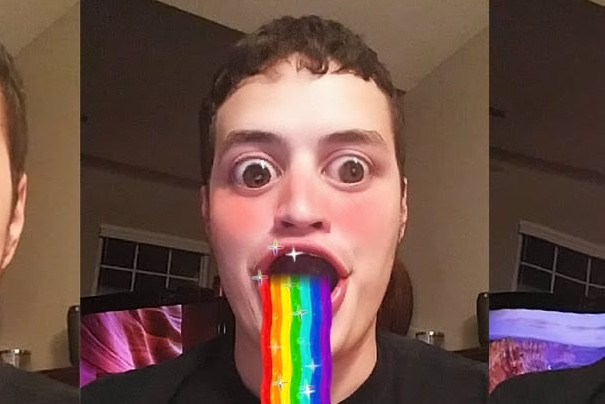
\includegraphics[width=\linewidth]{snapchat.jpg}
        \caption{Aplicação \textit{Snapchat}}\label{fig:snapchat}
    \end{subfigure}

    \begin{subfigure}[b]{.45\linewidth}
        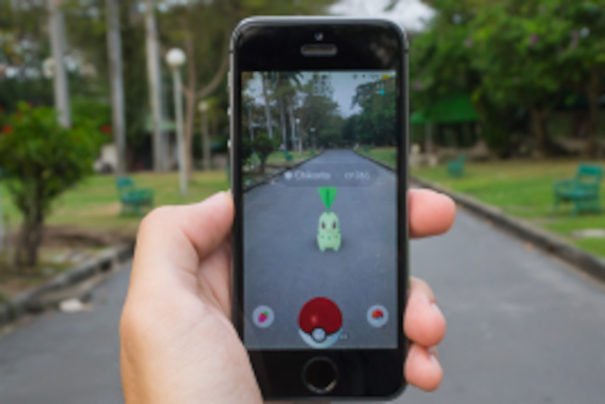
\includegraphics[width=\linewidth]{pokemongo.png}
        \caption{Aplicação \textit{Pokémon GO}}\label{fig:pokemongo}
    \end{subfigure}
    \begin{subfigure}[b]{.45\linewidth}
        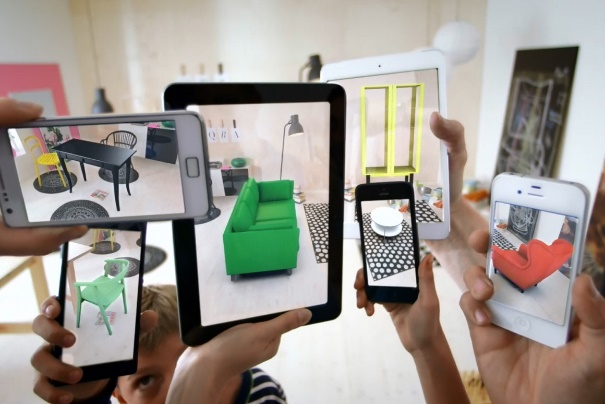
\includegraphics[width=\linewidth]{ikea.png}
        \caption{Aplicação \textit{IKEA}}\label{fig:ikea}
    \end{subfigure}
\caption{A Realidade Aumentada na atualidade.}
\label{fig:applications0}
\end{figure}

Esta “mistura” da realidade com o virtual será visualizada pelo utilizador no próprio display do \textit{smartphone}. Será que no futuro continuará a ser assim? Ou será uma experiência mais real e imersiva? Será que as aplicações serão também mais úteis?

\section{Aplicações - Futuro}
No futuro, com o crescente investimento no desenvolvimento desta tecnologia, tudo aponta para que a \ac{ra} esteja mais presente não só nos jogos, mas também em áreas onde atualmente tem pouca expressão (mas muito potencial) tais como a medicina, a engenharia e arquitetura, a educação e o ramo da logística. 

\subsection{Videojogos}
Na área dos jogos, com o avanço dos telemóveis e a vulgarização de, por exemplo, óculos holográficos, os jogos poderão ser muito mais complexos e, mesmo com a componente virtual, promover uma ligação maior com a realidade.

\subsection{Medicina}
Na área da medicina, ainda com pouca expressividade, a \ac{ra} já vai dando os seus primeiros passos, começando a ser utilizada para preparar e executar procedimentos cirúrgicos.

Atualmente, por exemplo, os doutores Jonathan Silva e Jennifer Silva da Universidade de Washington criaram um procedimento cirúrgico chamado \ac{elvis} que cria uma imagem tridimensional em tempo real do coração do paciente. Este procedimento reduz as chances de ser necessário repetir a operação no futuro. Estima-se, portanto, que se poupem cerca de 370 milhões de dólares anualmente.\cite{staff_2021}

\begin{figure}[H]
    \centering
    \begin{subfigure}{.5\textwidth}
      \centering
      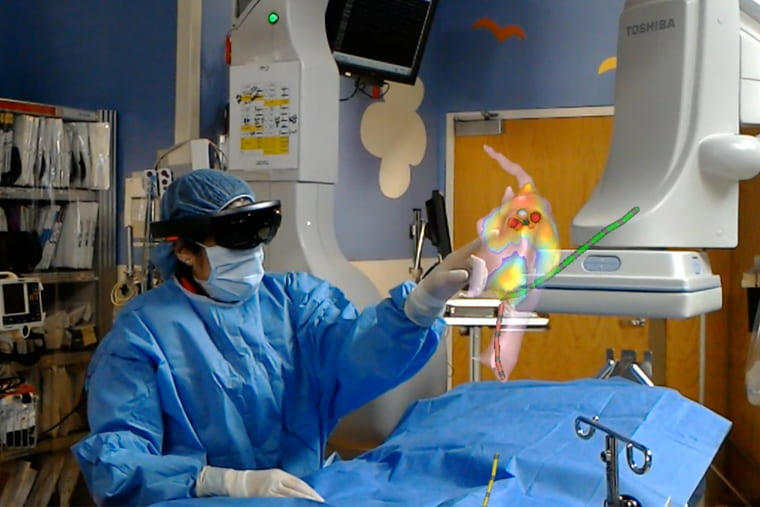
\includegraphics[width=17em]{medicin0.jpg}
      \label{Fig:medicin0}
    \end{subfigure}%
    \begin{subfigure}{.5\textwidth}
      \centering
      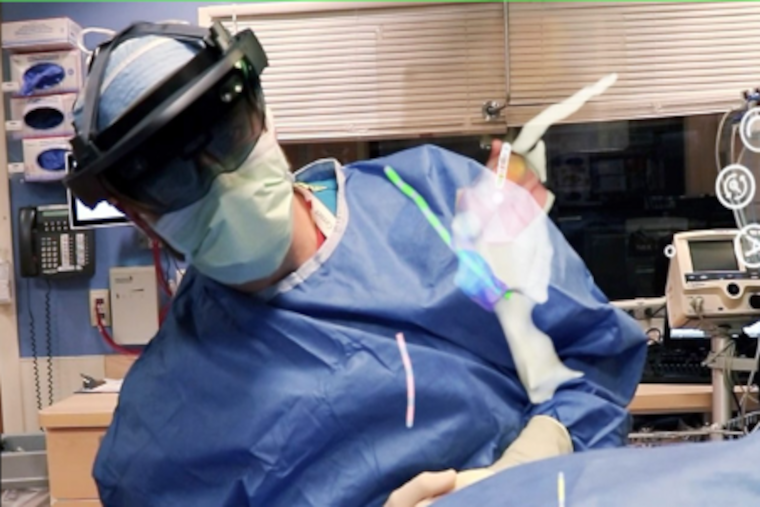
\includegraphics[width=17em]{medicin1.png}
      \label{Fig:medicin1}
    \end{subfigure}
    \caption{Utilização do procedimento ĒLVIS}
    \label{Fig:medicin}
\end{figure}

Mas com o espectável crescimento e desenvolvimento desta tecnologia, a tendência é que para num futuro próximo a \ac{ra} se torne no "braço direito" de todos os cirurgiões e pesquisadores nesta área.

\subsection{Engenharia e Arquitetura}
Na engenharia e na arquitetura, com a \ac{ra} mais difundida, além do aumento do ritmo do planeamento e da redução de custos, será mais fácil partilhar ideias de projetos e será possível pré visualizar o aspeto de uma casa no local onde esta será construída, permitindo que os proprietários e arquitetos tenham uma ideia mais fiel à realidade.

\begin{figure}[H]
    \centering
    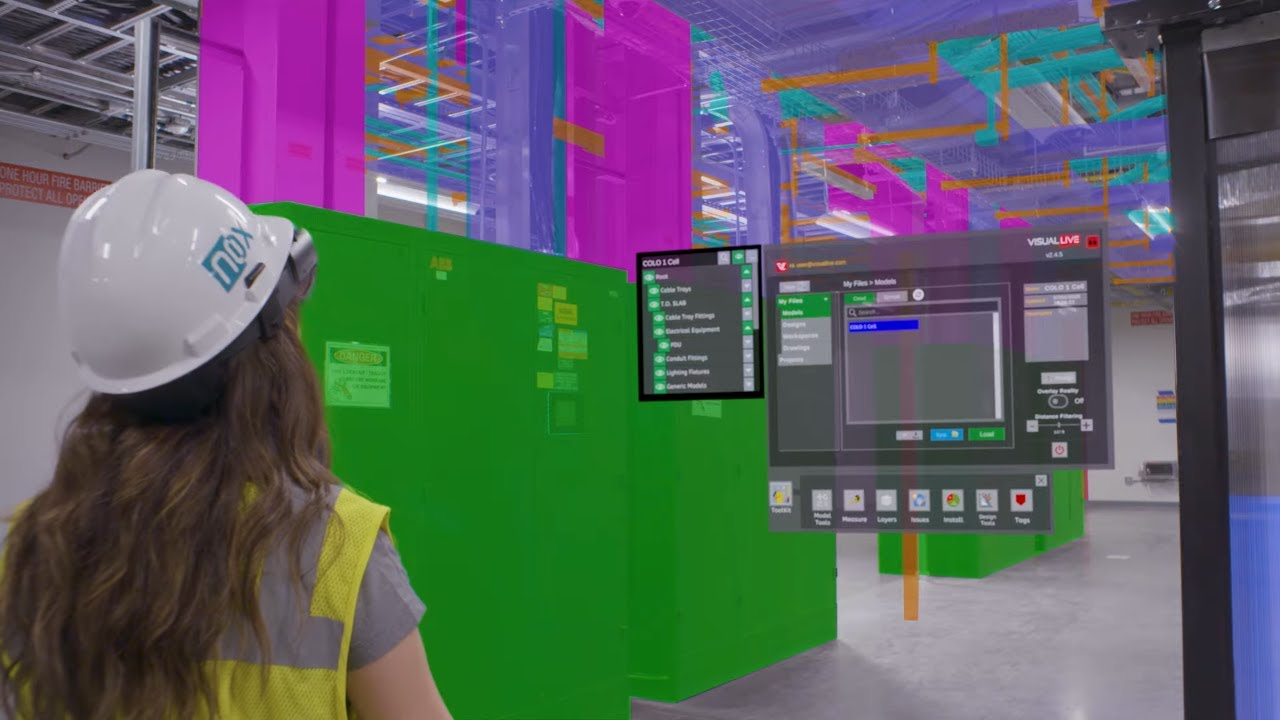
\includegraphics[width=20em]{arquieng.jpg}
    \caption{Pré visualização de estruturas.}
    \label{Fig:arquieng}
\end{figure}

\subsection{Educação}
A realidade virtual pode vir a ser utilizada até mesmo na educação com a sobreposição de informação virtual na forma de textos, imagens e animações, facilitando e ajudando na compreensão dos conteúdos, por exemplo, com a criação de manuais escolares interativos.

\begin{figure}[H]
    \centering
    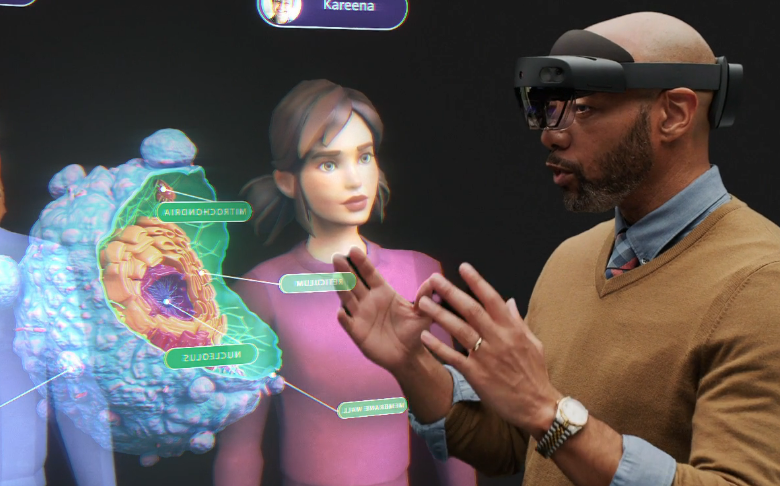
\includegraphics[width=20em]{education.png}
    \caption{Modelo 3D interativo de uma célula.}
    \label{Fig:education}
\end{figure}

Além de transformar conteúdo estático em conteúdo dinâmico, aulas que recorram à \ac{ra} irão gerar mais interesse, motivação e atenção por parte dos alunos.\cite{sinha_2021}

\subsection{Logística}
Se na atualidade as compras online já representam grande parte da atividade online, no futuro ainda irão representar uma maior parte. Com esse aumento da demanda, os centros logísticos irão sofrer uma grande sobrecarga.

A solução para a sobrecarga dos centros de distribuição e armazéns poderá passar por equipar os funcionários que neles trabalham com dispositivos de \ac{ra} de modo a aumentar a sua eficiência.

\begin{figure}[H]
    \centering
    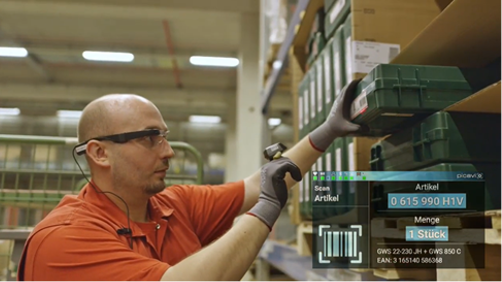
\includegraphics[width=20em]{logistics.png}
    \caption{Utilização de Realidade Aumentada num armazém logístico.}
    \label{Fig:logistics}
\end{figure}

Devido à situação pandémica, as empresas de transportes aéreos de mercadorias sentiram uma crescente sobrecarga com o aumento do volume de compras online. Assim, investiram em tecnologias de \ac{rv} e de \ac{ra} que, segundo a agência de notícias \ac{abn}, ajudaram as empresas a ultrapassar as dificuldades sentidas.\cite{moody_2020}

\section{Desafios e limitações}
!!!TODO!!!

%%% ÓCULOS HOLOGRÁFICOS %%%
\chapter{Óculos Holográficos}
\label{chap.oculos-holograficos}
Neste capítuo irá-se falar sobre um dispositivo que permite que a \ac{ra} seja mais imersiva: os Óculos Holográficos, demonstrando a sua utilidade para o quotidiano e as vantagens que a sua utilização trará para o dia a dia.

Também se fará um balanço do panorama atual destes dispositivos referindo as principais empresas interessadas no seu desenvolvimento e aprimoramento.

\section{Conceito}
O conceito dos óculos holográficos surgiu ao mesmo tempo que a criação do conceito de \ac{ra} por Thomas Caudell.

O objetivo que se tem tentado alcançar para cada nova geração destes dispositivos é fazer com que se pareçam óculos comuns, mas que nas suas lentes seja apresentada uma imagem holográfica que se funda com o ambiente real.

Graças ao rápido desenvolvimento de outras áreas da tecnologia, tem sido possível criar \textit{designs} cada vez mais simples e minimalistas e, efetivamente, os óculos holográficos têm ficado mais discretos, como comprova a Fig.~\ref{Fig:oculos}.

\begin{figure}[H]
    \centering
    \begin{subfigure}{.5\textwidth}
      \centering
      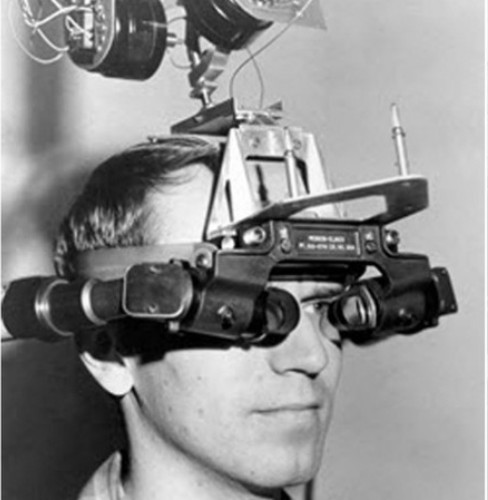
\includegraphics[height=11em]{firsthmd.jpg}
      \label{Fig:hmd}
    \end{subfigure}%
    \begin{subfigure}{.5\textwidth}
      \centering
      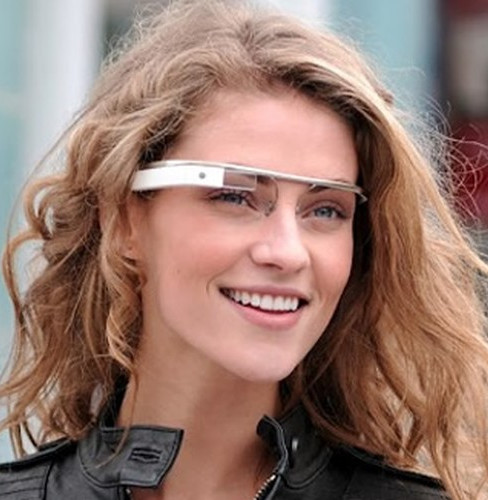
\includegraphics[height=11em]{googleglass.jpg}
      \label{Fig:googleglass}
    \end{subfigure}
    \caption{O primeiro \ac{hmd} Vs. \textit{Google Glass}}
    \label{Fig:oculos}
\end{figure}

\section{Panorama atual}
A \ac{ra} e as formas de a tornarem mais imersiva através dos óculos têm vindo a ser alvo de estudo por parte de grandes empresas no ramo da tecnologia que a pretendem implementar em diversas áreas, sejam estas no ramo da engenharia, da saúde, da arquitetura e até da educação.

Toda esta pesquisa levou ao desenvolvimento de hardware específico para que, de forma intuitiva e prática, fosse possível usar a \ac{ra} como “braço-direito” nas tarefas no dia a dia de trabalho. Assim, empresas como a \textit{Epson}, a \textit{Vuzix}, a \textit{Solos}, a \textit{Google}, a \textit{Microsoft}, entre outras, têm vindo a desenvolver óculos que permitem ao utilizador utilizar a \ac{ra} na sua atividade profissional.

Apesar de existir muita pesquisa e estarem grandes empresas envolvidas, as opções de equipamentos que permitem visualizar a \ac{ra} e interagir com o virtual de forma satisfatória são um tanto quanto limitadas. Existem, por exemplo, os \textit{Google Glasses} e os \textit{Epson BT Smart Glasses} porém, são muito rudimentares quando comparados aos óculos \textit{HoloLens 2} da \textit{Microsoft}.

%%% MICROSOFT HOLOLENS 2 %%%
\chapter{Microsoft \textit{HoloLens 2}}
\label{chap.microsoft-hololens-2}
No 4º capítulo apresentamos o Microsoft \textit{Hololens 2}. Um exemplo dum produto que nos permite imergir na \ac{ra} e que pode ser adquirido por qualquer pessoa para poder usufruir em qualquer lado.

Abordaremos as principais características do produto, o seu objetivo principal para o uso diário e o seu revolucionário \textit{design} que revolucionou o mercado por ser tão imersivo, e em simultâneo tão confortável.

\section{Proposta do produto}
A Microsoft apresenta ao público um novo e revolucionário dispositivo de realidade aumentada. Através de um design minimalista e moderno, o “HoloLens 2” promete ser mais eficiente que a sua versão anterior e que todos os seus concorrentes. 

É apresentado como um produto que irá servir para todas as idades, para qualquer uso que nos seja útil, e desta vez com um formato mais confortável, para poder ser utilizado diversas horas sem causar desconforto ao utilizador e poder tirar o maior proveito sem qualquer incómodo nem constrangimento.

\begin{quote}
    "\emph{Não existirá nenhum produto que compita com o nosso nos próximos dois a três anos e que possa garantir o nível de fidelidade que apresentamos.}"
\end{quote}
\begin{flushright}
    Zulfi Alan, gerente geral de engenharia ótica
\end{flushright}


\section{Design e principais características}
a. Campo de visão
Uma das maiores críticas direcionadas à primeira versão destes óculos estava relacionada com o pequeno campo de visão. Assim, a segunda versão foi desenhada para permitir apresentar um maior campo de visão aumentando, então, a “imersão” neste ambiente misto.

b. Resolução
Visto que o objetivo de produtos como este prende-se pela inserção de elementos virtuais na realidade existiu a grande necessidade de aumentar a resolução dos hologramas. Assim, através de uma complexa projeção a laser que guia a luz diretamente para a retina do utilizador, o \textit{“display”} transparente emite uma imagem holográfica de resolução 2K em cada um dos olhos do utilizador fazendo com que os hologramas parecem mais naturais e reais.

c. Ajuste interpupilar
Cada pessoa tem características faciais diferentes o que implica a necessidade de um ajuste de forma a que a imagem fique adequada e não cause desconforto ao utilizador. Os HoloLens recorrem a pequenos sensores no interior dos óculos para medir a distância entre as pupilas dos nossos olhos de modo a que então a imagem seja corretamente ajustada.

d. \textit{“Mixed Reality”}
\textit{Mixed Reality} é, segundo a Microsoft o termo mais correto para caracterizar o tipo de \ac{ra} a que estes óculos se destinam: uma realidade onde os elementos virtuais se encontram perfeitamente integrados. Com pequenos sensores posicionados nos óculos e através de um sistema de localização e análise dos movimentos das mãos do utilizador é possível manipular os hologramas de forma intuitiva. Para além disto, um algoritmo de inteligência artificial analisa todo o cenário em redor do utilizador e identifica todos os elementos presentes na sala permitindo que o computador identifique superfícies e locais onde poderá ou não projetar um holograma.


\section{Público Alvo}
O grande propósito destes óculos é o aumento da produtividade de cada uma das pessoas que os utiliza.
Para pessoas comuns, este produto poderá ter pouca ou nenhuma utilidade, mas, por outro lado, engenheiros e artistas, por exemplo, podem ver este produto como uma ferramenta muito promissora que poderá facilitar o processo de criação de algo.

%%% CONCLUSÕES %%%
\chapter{Conclusões}
\label{chap.conclusao}

Ao contrário do que se possa imaginar, a \ac{ra} não irá ficar limitada apenas ao contexto empresarial ou militar — todas as evoluções desta tecnologia irão ditar o estilo de vida do ser humano daqui a umas décadas, já que terá um impacto significativo no quotidiano de uma pessoa comum.

Neste trabalho desenvolvemos e explicamos o conceito de \ac{ra} através da comparação desta tecnologia com a \ac{rv}, da explicação da sua origem e as eventuais utilizações que esta tem e terá no nosso mundo. Apresentamos um dos dispositivos de \ac{ra} mais promissores na atualidade (Óculos Holográficos) exemplificando diversas utilidades práticas que estes têm. Por fim analisamos e demonstramos o produto atual de \ac{ra} que consideramos ser o mais revolucionário, os “Microsoft \textit{HoloLens 2}”. Este foi um trabalho que nos permitiu descobrir e desvendar o atual paradigma desta tecnologia e da qual nos consideramos fãs. Foi possível ainda perceber as limitações da \ac{rv} em relação ao mundo real e concluir que o futuro apresenta-se muito mais promissor para a \ac{ra}. Acreditamos que com a aposta de grandes empresas como a Google e a Microsoft na \ac{ra}, em um curto espaço de tempo, a maioria das atividades comerciais irão fazer uso desta tecnologia. Dado isto não será improvável o surgimento de novas empresas e novos produtos que irão concorrer frente a frente com os que já existem atualmente, permitindo um desenvolvimento ainda maior desta tecnologia fazendo ainda com que num futuro próximo, a utilização desta tecnologia possa vir a ser utilizada no quotidiano de pessoas comuns e não apenas no ambiente corporativo.

\chapter*{Contribuições dos autores}
Ambos participámos ativamente e com empenho, procurando contribuir para a realização dum trabalho com bom conteúdo, que possa transmitir boa informação para o leitor, e, que seja elaborado com uma boa apresentação para se tornar mais apelativo.

No geral houve esforço por ambas as partes para o bem do trabalho, tendo várias horas de pesquisa e aprendizagem investidas, mas o MG demonstrou maior empenho e dedicação tanto à aparência do trabalho como à quantidade de informação útil disponível neste. Graças a isso o trabalho foi concordado que o trabalho foi aproximadamente distribuido em: 60\% para \ac{mg} e 40\% para \ac{ds}.



%%% ACRÓNIMOS %%%
\chapter*{Acrónimos}
\begin{acronym}
\acro{abn}[ABN]{\textit{Aviation Business News}}
\acro{elvis}[ĒLVIS]{\textit{Enhanced Electrophysiology Visualization and Interaction System}}
\acro{hmd}[HMD]{\textit{Head-Mounted-Display}}
\acro{leci}[LECI]{Licenciatura em Engenharia de Computadores e Informática}
\acro{mg}[MG]{Miguel Vila}
\acro{ds}[DS]{Diogo Silva Gomes Pais e Silva}
\acro{ra}[RA]{Realidade Aumentada}
\acro{rm}[RM]{Realidade Mista}
\acro{rv}[RV]{Realidade Virtual}
\acro{ua}[UA]{Universidade de Aveiro}
\acro{iei}[IEI]{Introdução à Engenharia Informática}
\end{acronym}

%%% BIBLIOGRAFIA %%%
\printbibliography

\end{document}